\documentclass[11pt]{article}

\usepackage[a4paper,margin=1in]{geometry}
\usepackage[T1]{fontenc}
\usepackage[utf8]{inputenc}
\usepackage{lmodern}
\usepackage{microtype}
\usepackage{amsmath,amssymb,amsthm,mathtools}
\usepackage{booktabs,array,graphicx,float}
\usepackage[section]{placeins}
\usepackage{enumitem}
\usepackage[numbers,sort&compress]{natbib}
\usepackage{xcolor,xurl}
\usepackage[colorlinks=true,linkcolor=blue!55!black,citecolor=blue!55!black,urlcolor=blue!55!black]{hyperref}
\usepackage[nameinlink,noabbrev]{cleveref}

\setlength{\parindent}{1.4em}
\setlength{\parskip}{0.12em}
\setlist{itemsep=0.25em,topsep=0.35em}
\newtheorem{theorem}{Theorem}[section]
\newtheorem{proposition}[theorem]{Proposition}
\newtheorem{lemma}[theorem]{Lemma}
\newtheorem{corollary}[theorem]{Corollary}
\theoremstyle{remark}
\newtheorem{remark}[theorem]{Remark}

\newcommand{\Id}{\mathrm I}
\newcommand{\cB}{\mathcal B}
\newcommand{\cK}{\mathcal K}
\newcommand{\cP}{\mathcal P}
\newcommand{\cW}{\mathcal W}
\newcommand{\BV}{\mathrm{BV}}
\newcommand{\norm}[1]{\left\lVert #1\right\rVert}
\newcommand{\len}{\operatorname{len}}

\title{Strong--Weak Adaptive Cutoff Transfer for Intrinsic Riesz Factors\\
\large Sandwiched Functional Calculus, Midpoint--Ulam Contour Inheritance,
and a Fixed-Window Route No-Go}
\author{Liang Wang}
\date{July 2026}

\begin{document}
\maketitle

\begin{abstract}
The factor-aware intrinsic-identification theorem for a small-noise quadratic
Markov family left one analytic premise: a row-normalized adaptive Gaussian
cutoff must remain small after the finite matrix recomputes its own Perron
and parity Riesz factors.  A direct Hilbert-space resolvent argument cannot
close this premise.  Endpoint spikes force the complete fixed-contour
$L^2$ resolvent to grow at least as
$\sqrt{\log(1/\sigma)}$.

We bypass that obstruction with a two-sided transfer identity.  If a contour
$\Gamma$ avoids zero, then
\[
 \Pi(T;\Gamma)=\frac1{2\pi i}\int_\Gamma
 z^{-2}T(z-T)^{-1}T\,dz,
 \qquad
 \cW(T;\Gamma)=\frac1{2\pi i}\int_\Gamma
 z^{-1}T(z-T)^{-1}T\,dz.
\]
The two outer transfer operators convert a strong-space contour resolvent
into an $L^1\to L^2$ Riesz bound.  For reference and perturbed operators,
the sandwiched defect is bounded by
\[
 D\le \rho MR+SM\widetilde M\tau_1R+S\widetilde M\tau_0,
\]
where $M,\widetilde M$ are strong-space resolvent bounds,
$R=\norm T_{L^1\to\cB}$, $S=\norm{\widetilde T}_{L^1\to L^2}$,
$\rho=\norm{T-\widetilde T}_{L^1\to L^2}$, and
$\tau_0,\tau_1$ are the $L^1\to\cB$ and $\cB\to\cB$ defects.

We first bridge the exact Ulam operator and the full discretely normalized
midpoint family.  Conditioned folded-Gaussian derivatives give row
$L^1$ error $O(h^2\sigma^{-2})$ and piecewise-BV error
$O(h\sigma^{-2})$.  Hence the established strong-space peripheral contours
pass to the midpoint family on every $h=o(\sigma^2)$ schedule.  For a cutoff
$L_\kappa(h)=\max\{L_0,\sqrt{2\kappa\log(1/h)}\}$, a distribution-free
row-mass argument yields the sufficient threshold $\kappa\ge7/4$.
Using the Gaussian tail shape sharpens the Riesz defect to
\[
 \norm{\Delta\Pi}+\norm{\Delta\cW}
 =O(h^\kappa\sigma^{-5/2}),
\]
and lowers the sufficient all-schedule threshold to $\kappa\ge5/4$.
The archived choice $\kappa=2$ therefore gives $o(\sigma^{3/2})$ on every
$h=o(\sigma^2)$ schedule.  Fixed $L$ fails to vanish through this
strong--BV route; this is not a theorem that the actual projectors diverge.

A four-level midpoint--Ulam audit and the five-scale intrinsic-factor data
from the preceding paper support the mechanisms.  A separate 256-bit Arb
run audits the scalar ledgers.  These computations are not production-scale
interval eigensolvers.  The result closes the analytic adaptive
Riesz/cutoff premise, while the dyadically uniform Hardy--Stein trace budget
remains open.
\end{abstract}

\noindent\textbf{Keywords:} Riesz projection; strong--weak stability;
Ulam approximation; Gaussian cutoff; nonnormal perturbation; small noise.

\medskip
\noindent\textbf{MSC 2020:} 47A55; 37M25; 47B65; 65R20; 37A30.

\section{Introduction}

The small-noise intrinsic determinant program has now reduced its
sparse/full interface to a precise nonnormal question.  RH-53 gave a
deterministic all-column Hardy-tail certificate and the exact-real adaptive
Gaussian matrix bridge \citep{WangHardyTail2026}.  RH-54 then propagated
operator, coupling, projector, and weighted-Riesz defects through normalized
Hardy triples and growing horizons \citep{WangFactorAware2026}.  The only
missing input in that composition was an analytic modulus for the matrix's
\emph{recomputed} intrinsic Riesz factors.

The naive solution is unavailable.  For a common $L^2$ contour one may use
two complete resolvents and the operator defect, as in the original
weighted-Riesz perturbation theorem \citep{WangWeightedRiesz2026}.  However,
the endpoint square-root densities imply
\[
 \norm{\Pi_{\pm,\sigma}}_{L^2\to L^2}
 =\Theta\!\left(\sqrt{\log(1/\sigma)}\right),
\]
so a uniform $O(1)$ fixed-contour $L^2$ resolvent is impossible
\citep{WangLogConditioning2026}.  This is a structural obstruction, not a
defect of the numerical method.

The strong--weak perturbation framework used to identify the Perron and
parity branches provides a different route.  The conditioned folded-Gaussian
transfer operator acts on a postcritical tower/spike space $\cB$, with
$L^1$ as weak norm and fixed isolating contours inherited from the
deterministic branches \citep{WangBoundaryLayer2026,WangFactorTransfer2026}.
Gaussian smoothing then maps weak inputs to $L^2$.  The only missing algebra
is to place that smoothing on both sides of the resolvent.  The identities in
the abstract do exactly this.

The paper has four analytic contributions.

\begin{enumerate}[leftmargin=2em]
 \item It proves the sandwiched functional-calculus identities and a
 three-term strong--weak perturbation bound for both the unweighted
 projector and weighted Riesz term.
 \item It supplies the midpoint--Ulam comparison omitted from the previous
 strong--weak factor theorem, including the conditioned normalizer and a
 piecewise-BV strong estimate.
 \item It converts the exact twice-the-tail row identity into a generic
 mass-only adaptive theorem with sufficient threshold $\kappa=7/4$.
 \item It exploits the actual Gaussian boundary shape to remove the
 artificial cell-jump loss, yielding the sharper threshold $\kappa=5/4$
 and an $o(\sigma^{3/2})$ defect for the archived $\kappa=2$ rule.
\end{enumerate}

Both thresholds are sufficient for their respective proof ledgers.  Neither
is asserted to be necessary for actual Riesz stability.  Likewise, the
fixed-window negative statement concerns this strong--BV proof route only.

Three evidence levels are kept separate.
\begin{description}[leftmargin=3.6cm,style=nextline]
 \item[Analytic theorem]
 Kernel derivative bounds, midpoint--Ulam transfer, strong-space contour
 inheritance, and the sandwiched Riesz modulus.
 \item[Binary64 diagnostic]
 Four midpoint--Ulam grids and five inherited dense intrinsic-factor scales.
 \item[Arb arithmetic audit]
 256-bit evaluation of the scalar tail and sandwich formulas, not an
 interval eigensolver for the production matrix.
\end{description}

\section{Operator conventions and strong--weak contours}

Let $I=[0,1]$, $u=u_{\rm c}$ be the first quadratic band-merging parameter,
and $f(x)=1-ux^2$.  Put
\[
 \phi_\sigma(t)=\frac{e^{-t^2/(2\sigma^2)}}{\sqrt{2\pi}\sigma},
 \qquad
 g_\sigma(x,y)=\phi_\sigma(y-f(x))+\phi_\sigma(-y-f(x)),
\]
\[
 Z_\sigma(x)=\int_0^1g_\sigma(x,y)\,dy,
 \qquad
 k_\sigma(x,y)=\frac{g_\sigma(x,y)}{Z_\sigma(x)}.
\]
The density transfer operator is
\begin{equation}
 (\cP_\sigma q)(y)=\int_I k_\sigma(x,y)q(x)\,dx.
 \label{eq:density-operator}
\end{equation}
Its transpose is the Markov operator on observables.  We work on the density
side because the tower/spike space $\cB$ embeds compactly into $L^1$.

Normalize the strong norm so that
$\norm q_1\le\norm q_{\cB}$.  The established uniform Lasota--Yorke
estimate has the form
\begin{equation}
 \norm{\cP_\sigma^m q}_{\cB}
 \le A\vartheta^m\norm q_{\cB}+B\norm q_1,
 \qquad 0<\vartheta<1,
 \label{eq:lasota-yorke}
\end{equation}
with constants independent of small $\sigma$.  Keller--Liverani stability
then supplies disjoint fixed-geometry contours $\Gamma_+$ and $\Gamma_-$
around the branches converging to $1$ and $-1$ \citep{KellerLiverani1999}.
In particular,
\begin{equation}
 \sup_{z\in\Gamma_+\cup\Gamma_-}
 \norm{(z-\cP_\sigma)^{-1}}_{\cB\to\cB}\le M
 \label{eq:strong-resolvent}
\end{equation}
for all sufficiently small $\sigma$.

The $L^2$ analogue of \eqref{eq:strong-resolvent} is false uniformly.  The
proof below never assumes it.

\section{Sandwiched Riesz functional calculus}

Let $T$ be bounded on a Banach space, and let $\Gamma\subset\rho(T)$ be a
positively oriented rectifiable contour whose interior avoids the spectral
point zero.  Define
\[
 \Pi(T;\Gamma)=\frac1{2\pi i}\int_\Gamma(z-T)^{-1}\,dz,
 \qquad
 \cW(T;\Gamma)=T\Pi(T;\Gamma).
\]

\begin{lemma}[Two-sided transfer identities]
\label{lem:sandwich-identities}
If $0$ lies outside $\Gamma$, then
\begin{align}
 \Pi(T;\Gamma)
 &=\frac1{2\pi i}\int_\Gamma
 z^{-2}T(z-T)^{-1}T\,dz,
 \label{eq:projector-sandwich}\\
 \cW(T;\Gamma)
 &=\frac1{2\pi i}\int_\Gamma
 z^{-1}T(z-T)^{-1}T\,dz.
 \label{eq:weighted-sandwich}
\end{align}
\end{lemma}

\begin{proof}
Because $T$ commutes with its resolvent,
\[
 T(z-T)^{-1}T=z^2(z-T)^{-1}-z\Id-T.
\]
After multiplication by $z^{-2}$, the last two terms are
$-z^{-1}\Id-z^{-2}T$.  Their contour integrals vanish because zero lies
outside $\Gamma$.  This proves \eqref{eq:projector-sandwich}.  Multiplying
the same identity by $z^{-1}$ leaves
$z(z-T)^{-1}-\Id-z^{-1}T$; its integral is
$T\Pi(T;\Gamma)$ because the last two terms again integrate to zero.
\end{proof}

We now state the abstract perturbation estimate in the scale needed below.
Assume $\cB\hookrightarrow L^1$ and let $T,\widetilde T$ act consistently on
$L^1$ and $\cB$.  Put $R_T(z)=(z-T)^{-1}$ and similarly for
$\widetilde T$.

\begin{theorem}[Strong--weak sandwich perturbation]
\label{thm:sandwich}
Suppose, uniformly on $z\in\Gamma$,
\begin{align*}
 \norm{R_T(z)}_{\cB\to\cB}&\le M,&
 \norm{R_{\widetilde T}(z)}_{\cB\to\cB}&\le\widetilde M,\\
 \norm T_{L^1\to\cB}&\le R,&
 \norm{\widetilde T}_{L^1\to L^2}&\le S,
\end{align*}
and define
\begin{align*}
 \rho&=\norm{T-\widetilde T}_{L^1\to L^2},\\
 \tau_0&=\norm{T-\widetilde T}_{L^1\to\cB},&
 \tau_1&=\norm{T-\widetilde T}_{\cB\to\cB}.
\end{align*}
Then
\begin{equation}
 \norm{TR_T(z)T-\widetilde T R_{\widetilde T}(z)\widetilde T}_{L^1\to L^2}
 \le D,
 \label{eq:sandwich-defect}
\end{equation}
where
\begin{equation}
 \boxed{D=\rho MR+SM\widetilde M\tau_1R+S\widetilde M\tau_0.}
 \label{eq:D}
\end{equation}
Consequently
\begin{align}
 \norm{\Pi(T;\Gamma)-\Pi(\widetilde T;\Gamma)}_{L^1\to L^2}
 &\le\frac{\len(\Gamma)}{2\pi}
 \max_{z\in\Gamma}|z|^{-2}D,
 \label{eq:projector-defect}\\
 \norm{\cW(T;\Gamma)-\cW(\widetilde T;\Gamma)}_{L^1\to L^2}
 &\le\frac{\len(\Gamma)}{2\pi}
 \max_{z\in\Gamma}|z|^{-1}D.
 \label{eq:weighted-defect}
\end{align}
\end{theorem}

\begin{proof}
Add and subtract the two intermediate products:
\begin{align*}
 TR_TT-\widetilde T R_{\widetilde T}\widetilde T
 ={}&(T-\widetilde T)R_TT\\
 &+\widetilde T(R_T-R_{\widetilde T})T
 +\widetilde T R_{\widetilde T}(T-\widetilde T).
\end{align*}
Because $\norm q_1\le\norm q_{\cB}$, the $L^1\to L^2$ outer bounds also
apply to strong-space inputs.  The first and third terms therefore have
bounds $\rho MR$ and
$S\widetilde M\tau_0$.  The resolvent identity
\[
 R_T-R_{\widetilde T}=R_T(T-\widetilde T)R_{\widetilde T}
\]
may equivalently be written with the resolvents interchanged; using the
placement consistent with the displayed product gives the middle bound
$SM\widetilde M\tau_1R$.  Integrating
\cref{eq:projector-sandwich,eq:weighted-sandwich} proves the result.
\end{proof}

\begin{remark}
The theorem is stated as an $L^1\to L^2$ estimate.  Since the physical
interval has unit measure, $L^2\hookrightarrow L^1$ contractively, so it is
also an $L^2\to L^2$ estimate.  On a finite equal-cell space, the standard
isometric density lift identifies the latter with the Euclidean matrix
norm.  Thus \cref{eq:projector-defect,eq:weighted-defect} are exactly the
intrinsic defects consumed by RH-54.  No complete global $L^2$ resolvent
appears.
\end{remark}

\section{From exact Ulam to the midpoint family}

Let $I_i=[ih,(i+1)h)$, $x_i=(i+1/2)h$, and let $E_h$ be equal-cell
conditional expectation.  The exact Ulam density operator is
\[
 U_{h,\sigma}=E_h\cP_\sigma|_{V_h}.
\]
Its row-stochastic observable transpose has entries
\begin{equation}
 (U^{\rm obs}_{h,\sigma})_{ij}
 =\frac1h\int_{I_i}\int_{I_j}k_\sigma(x,y)\,dy\,dx.
 \label{eq:exact-ulam}
\end{equation}
The full midpoint matrix used in the numerical branch is
\begin{equation}
 (P^{\rm mid}_{h,\sigma})_{ij}
 =\frac{g_\sigma(x_i,x_j)}{\sum_mg_\sigma(x_i,x_m)}.
 \label{eq:midpoint-matrix}
\end{equation}
These are not identical and must not be conflated.

\begin{lemma}[Conditioned folded-Gaussian derivatives]
\label{lem:kernel-derivatives}
For all sufficiently small $\sigma$,
\begin{align}
 \sup_{x\in I}\int_I
 \bigl(|\partial_{xx}k_\sigma(x,y)|
      +|\partial_{yy}k_\sigma(x,y)|\bigr)\,dy
 &\le C\sigma^{-2},
 \label{eq:second-derivative-l1}\\
 \sup_{x\in I}\int_I|\partial_y k_\sigma(x,y)|\,dy
 &\le C\sigma^{-1}.
 \label{eq:first-derivative-l1}
\end{align}
For a target tail beginning at distance $L\sigma$, the first-variation
bound \eqref{eq:first-derivative-l1}, including its boundary jump, improves
to $C\sigma^{-1}e^{-L^2/2}$.
\end{lemma}

\begin{proof}
For an unconditioned Gaussian,
\[
 \int|\phi_\sigma'|=O(\sigma^{-1}),
 \qquad
 \int|\phi_\sigma''|=O(\sigma^{-2}).
\]
The $y$ derivatives follow by folding and restriction.  For $x$ derivatives,
the chain rule adds bounded factors $f'$ and $f''$.  It remains to control
$Z_\sigma^{-1}$.  The physical image $f(I)\subset[1-u,1]$ and the symmetric
conditioning interval $[-1,1]$ give $Z_\sigma\ge c_0>0$ uniformly for small
$\sigma$ (indeed $Z_\sigma^{-1}\le2+o(1)$); moreover
$Z_\sigma' =O(\sigma^{-1})$ and $Z_\sigma''=O(\sigma^{-2})$ after scaling
the boundary Gaussian.  Differentiating $g/Z$ therefore preserves the same
powers.  Finally, the target variation of one Gaussian tail is its boundary
height: integrating $|\phi_\sigma'|$ from $L\sigma$ to infinity gives
$\phi_\sigma(L\sigma)=C\sigma^{-1}e^{-L^2/2}$.  Folding changes only the
constant.
\end{proof}

\begin{theorem}[Midpoint--Ulam strong transfer]
\label{thm:midpoint-ulam}
Uniformly for $h/\sigma$ sufficiently small,
\begin{align}
 \max_i\sum_j
 |(P^{\rm mid}_{h,\sigma})_{ij}
  -(U^{\rm obs}_{h,\sigma})_{ij}|
 &\le Ch^2\sigma^{-2},
 \label{eq:midpoint-row}\\
 \norm{(P^{\rm mid}_{h,\sigma})^*-(U^{\rm obs}_{h,\sigma})^*}_{\cB_h\to\cB_h}
 &\le Ch\sigma^{-2}.
 \label{eq:midpoint-strong}
\end{align}
Here $\cB_h$ is the cellwise spike/BV lift with its inherited strong norm.
Consequently, on every schedule $h=o(\sigma^2)$, the fixed strong-space
contours of the exact Ulam family are also common contours for the full
midpoint family, with uniformly bounded strong resolvents.
\end{theorem}

\begin{proof}
Apply composite midpoint quadrature first in the target variable and then
in the source cell.  The vector-valued midpoint remainder is bounded in
row $L^1$ by $Ch^2$ times
\eqref{eq:second-derivative-l1}.  Replacing the continuum normalizer by the
discrete row sum is a quotient perturbation with the same order because both
normalizers are bounded below.  This proves \eqref{eq:midpoint-row}.

Lift a row difference to a cellwise-constant signed density.  Its $L^1$
part is \eqref{eq:midpoint-row}; the conservative jump variation costs one
factor $h^{-1}$.  The spike atoms are finite and cell averaging is
variation diminishing on their regular representatives
\citep{Li1976,BoyarskyGora1997}.  Hence
\eqref{eq:midpoint-strong} follows.

The right side tends to zero precisely when $h=o(\sigma^2)$.  A Neumann
series around the exact-Ulam strong resolvent then gives common contours and
a uniform midpoint resolvent upper.  This is the finite-space contour
inheritance required by \cref{thm:sandwich}.
\end{proof}

\section{Generic mass-only cutoff transfer}

Let $\widetilde P_{h,\sigma}^{(L)}$ be obtained from the full midpoint row
by omitting entries outside the archived support window and renormalizing.
In this and the next section, $T$ and $\widetilde T$ denote the density
transposes of the full and cutoff row-stochastic matrices.  Uniform row
bounds therefore become $L^1$ density-operator bounds by Minkowski's
inequality.
If the omitted full-row probability is $q_i$, then the exact identity of
RH-39 is
\begin{equation}
 \norm{\Delta\mathrm{row}_i}_{\ell^1}=2q_i.
 \label{eq:twice-tail}
\end{equation}
Put $Q_h=\max_iq_i$.

\begin{lemma}[Distribution-free cell lift]
\label{lem:mass-lift}
Without using any smoothness of the omitted entries,
\begin{align}
 \rho&\le2Q_hh^{-1/2},
 \label{eq:rho-generic}\\
 \tau_0+\tau_1&\le C(Q_h+Q_hh^{-1}).
 \label{eq:tau-generic}
\end{align}
\end{lemma}

\begin{proof}
The cellwise density lift of a row has $L^2$ norm at most its $L^1$ mass
divided by $\sqrt h$, proving \eqref{eq:rho-generic}.  A signed
cellwise-constant density with $L^1$ mass $2Q_h$ has total jump variation at
most $4Q_h/h$.  Adding the $L^1$ part gives \eqref{eq:tau-generic}.
\end{proof}

Gaussian smoothing gives
\begin{equation}
 R=O(\sigma^{-1}),
 \qquad
 S=O(\sigma^{-1/2}).
 \label{eq:smoothing-coarse}
\end{equation}
The first bound is a strong BV/spike norm; the second is the standard
$L^1\to L^2$ kernel estimate.  Since the strong contour resolvents are
uniform, \cref{thm:sandwich,lem:mass-lift} yield the following theorem.

\begin{theorem}[Mass-only adaptive Riesz modulus]
\label{thm:mass-only}
If $Q_h/h=o(1)$, the cutoff family inherits the two strong-space contours,
and for either contour
\begin{equation}
 \norm{\Delta\Pi}+\norm{\Delta\cW}
 =O\!\left(\frac{Q_h}{h\sigma^{3/2}}\right).
 \label{eq:mass-only-riesz}
\end{equation}
For
\[
 L_\kappa(h)=\max\{L_0,\sqrt{2\kappa\log(1/h)}\},
\]
the RH-39 Mills bound gives
\[
 Q_h=O\!\left(
 \frac{h^\kappa}{\sqrt{\log(1/h)}}
 \right),
\]
and hence
\begin{equation}
 \norm{\Delta\Pi}+\norm{\Delta\cW}
 =O\!\left(
 \frac{h^{\kappa-1}\sigma^{-3/2}}
 {\sqrt{\log(1/h)}}
 \right).
 \label{eq:generic-adaptive}
\end{equation}
On every strict schedule $h=o(\sigma^2)$ this tends to zero if
$\kappa\ge7/4$.  For the archived $\kappa=2$ it is
\begin{equation}
 O\!\left(\frac{h\sigma^{-3/2}}
 {\sqrt{\log(1/h)}}\right)=o(\sqrt\sigma).
 \label{eq:generic-kappa-two}
\end{equation}
\end{theorem}

\begin{proof}
In \eqref{eq:D}, the middle term dominates the generic ledger and has size
$O(\sigma^{-1/2}(Q_h/h)\sigma^{-1})$.  This proves
\eqref{eq:mass-only-riesz}.  The tail formula follows from
$e^{-L_\kappa(h)^2/2}=h^\kappa$ and Mills' ratio
\citep{WangCutoff2026}.

On a boundary power schedule $h\asymp\sigma^p$, $p>2$, the polynomial
exponent is $p(\kappa-1)-3/2$.  Its limiting worst case as $p\downarrow2$
is nonnegative exactly when $\kappa\ge7/4$; the logarithmic factor gives
decay at equality.  Equation \eqref{eq:generic-kappa-two} is immediate.
Moreover $Q_h/h=o(1)$ throughout this range, so the contour-inheritance
premise in the theorem is automatic.
\end{proof}

\section{Gaussian shape refinement}

The preceding theorem treats an omitted Gaussian row as an arbitrary signed
cell vector.  That creates the $Q_h/h$ jump penalty.  The actual cutoff
difference is much smoother: away from two support boundaries it is a
rescaled Gaussian tail plus a small multiple of the retained full row.

\begin{lemma}[Shape-aware cutoff norms]
\label{lem:shape-cutoff}
Let $L_h\ge L_0>0$ and assume $h/\sigma$ is small.  Then the full and
row-renormalized cutoff midpoint operators satisfy
\begin{align}
 \rho&=O(e^{-L_h^2/2}\sigma^{-1/2}),
 \label{eq:shape-rho}\\
 \tau_0+\tau_1&=O(e^{-L_h^2/2}\sigma^{-1}).
 \label{eq:shape-tau}
\end{align}
The constants are independent of $h$, $\sigma$, and the moving integer
support boundary.
\end{lemma}

\begin{proof}
For one row, split the difference into the omitted tail and the retained
renormalization term.  The tail $L^2$ density norm is bounded by the square
root of a Gaussian-square tail, giving
$Ce^{-L_h^2/2}\sigma^{-1/2}$ after weakening any additional Mills factor.
Its target variation is the integral of $|\partial_yk_\sigma|$ beyond
$L_h\sigma$, plus the two boundary jumps.  By
\cref{lem:kernel-derivatives}, both are
$O(e^{-L_h^2/2}\sigma^{-1})$.  The retained term is $q_i/(1-q_i)$ times the
full row; RH-39 gives $q_i=O(e^{-L_h^2/2}/L_h)$, while the full row has
$L^2$ scale $O(\sigma^{-1/2})$ and variation $O(\sigma^{-1})$.

The operator acts on densities, so its strong output norm is target
variation.  No source derivative of the moving support is required: one
integrates these uniform row-BV bounds against the input density.  The
integer support boundary itself contributes only the two target jumps just
estimated.  Thus no $1/h$ factor is paid.
\end{proof}

\begin{theorem}[Gaussian shape-aware Riesz modulus]
\label{thm:shape-riesz}
If $e^{-L_h^2/2}\sigma^{-1}=o(1)$, the cutoff family inherits the two
strong-space contours, and for either contour
\begin{equation}
 \boxed{
 \norm{\Delta\Pi}+\norm{\Delta\cW}
 =O(e^{-L_h^2/2}\sigma^{-5/2}).}
 \label{eq:shape-riesz}
\end{equation}
For the adaptive $L_\kappa(h)$,
\begin{equation}
 \norm{\Delta\Pi}+\norm{\Delta\cW}
 =O(h^\kappa\sigma^{-5/2}).
 \label{eq:shape-adaptive}
\end{equation}
Every strict $h=o(\sigma^2)$ schedule is therefore preserved if
\begin{equation}
 \boxed{\kappa\ge\frac54.}
 \label{eq:shape-threshold}
\end{equation}
For RH-39's $\kappa=2$ rule,
\begin{equation}
 \norm{\Delta\Pi}+\norm{\Delta\cW}
 =O(h^2\sigma^{-5/2})=o(\sigma^{3/2}).
 \label{eq:kappa-two-sharp}
\end{equation}
\end{theorem}

\begin{proof}
Insert \cref{eq:shape-rho,eq:shape-tau} and
\eqref{eq:smoothing-coarse} into \eqref{eq:D}.  The first term is
$O(e^{-L_h^2/2}\sigma^{-3/2})$; the middle term is
$O(e^{-L_h^2/2}\sigma^{-5/2})$; and the third is
$O(e^{-L_h^2/2}\sigma^{-3/2})$.  The middle term gives
\eqref{eq:shape-riesz}.

For $h\asymp\sigma^p$, $p>2$, the exponent in
\eqref{eq:shape-adaptive} is $p\kappa-5/2$.  It is nonnegative uniformly as
$p\downarrow2$ when $\kappa\ge5/4$; on a strict little-$o$ schedule the
threshold case tends to zero.  For $\kappa=2$,
$h^2\sigma^{-5/2}=o(\sigma^{3/2})$ because $h/\sigma^2\to0$.
At every $\kappa\ge5/4$, the strong defect
$h^\kappa\sigma^{-1}$ also tends to zero, so the contour-inheritance
premise is automatic.
\end{proof}

\begin{remark}[Sufficient, not necessary]
The values $7/4$ and $5/4$ are thresholds for two explicit proof routes.
They are not lower bounds on the true cutoff needed by the folded-Gaussian
Riesz projector.  Cancellations or more anisotropic strong norms could
improve them.
\end{remark}

\begin{proposition}[Fixed-window route no-go]
\label{prop:fixed-no-go}
If $L_h\equiv L<\infty$, neither the mass-only nor the Gaussian-shape
strong--weak ledger gives a vanishing full-kernel Riesz perturbation as
$\sigma\to0$.  In the shape ledger the strong cutoff proxy grows as
$e^{-L^2/2}\sigma^{-1}$ and the Riesz proxy as
$e^{-L^2/2}\sigma^{-5/2}$.
\end{proposition}

\begin{proof}
The Gaussian boundary height $e^{-L^2/2}$ is a fixed positive number.
Substitute it in \cref{eq:shape-tau,eq:shape-riesz}.
\end{proof}

\begin{remark}
This is only a no-go for the present norm route.  It does not assert that
the actual fixed-window projectors fail to converge, and it does not
contradict the extremely small fixed-eight-sigma defects on every archived
finite grid.
\end{remark}

\section{Numerical mechanism audit}

The first audit compares \eqref{eq:exact-ulam} and
\eqref{eq:midpoint-matrix} at $\sigma=0.08$.  Each source-cell integral is
evaluated by 12-point Gauss--Legendre quadrature.  The calculation is
binary64 and is not used to establish the theorem.

\begin{table}[H]
\centering
\small
\begin{tabular}{@{}rrrrrr@{}}
\toprule
$n$&$h$&max row $L^1$&ratio to $h^2\sigma^{-2}$&max lifted BV&ratio to $h\sigma^{-2}$\\
\midrule
32 &$3.1250\,10^{-2}$&$5.99398\,10^{-2}$&0.39282&1.19324&0.24438\\
64 &$1.5625\,10^{-2}$&$1.58147\,10^{-2}$&0.41457&0.33176&0.13589\\
128&$7.8125\,10^{-3}$&$4.01200\,10^{-3}$&0.42069&0.08382&0.06867\\
256&$3.9063\,10^{-3}$&$1.00868\,10^{-3}$&0.42307&0.02125&0.03481\\
\bottomrule
\end{tabular}
\caption{Binary64 midpoint--Ulam mechanism audit.  The row defect follows
the predicted second-order scale; the conservative strong theorem requires
only the weaker $O(h\sigma^{-2})$ envelope.}
\label{tab:midpoint-ulam}
\end{table}

We also reuse, by hash, RH-54's dense full-versus-sparse intrinsic-factor
audit.  It has $n\sigma=5.12$, dimensions $32,64,128,256,512$, and declared
cutoffs $L=5,6,8$.  For the intentionally stressed $L=5$ family:

\begin{table}[H]
\centering
\small
\begin{tabular}{@{}rrrrrr@{}}
\toprule
$\sigma$&$n$&$Q_h$ upper&actual $\Delta\Pi$&actual $\Delta\cW$&sum/shape envelope\\
\midrule
0.16&32 &$4.9655\,10^{-7}$&$1.8305\,10^{-8}$&$2.3658\,10^{-8}$&$1.3410\,10^{-3}$\\
0.08&64 &$4.9655\,10^{-7}$&$2.7670\,10^{-8}$&$3.7163\,10^{-8}$&$3.6626\,10^{-4}$\\
0.04&128&$4.9655\,10^{-7}$&$2.4205\,10^{-8}$&$2.3020\,10^{-8}$&$4.7163\,10^{-5}$\\
0.02&256&$4.9655\,10^{-7}$&$3.2570\,10^{-8}$&$2.9979\,10^{-8}$&$1.1043\,10^{-5}$\\
0.01&512&$4.9655\,10^{-7}$&$2.8136\,10^{-8}$&$2.6251\,10^{-8}$&$1.6973\,10^{-6}$\\
\bottomrule
\end{tabular}
\caption{Inherited binary64 intrinsic-factor stress audit.  The last column
uses the unit-constant power envelope and is descriptive, not a rigorous
constant comparison.}
\label{tab:factor-audit}
\end{table}

The maximum observed projector-plus-weighted defect is
$6.49\times10^{-8}$.  At $L=6$ it is about $10^{-10}$ beyond the smallest
dimension, and at $L=8$ it reaches binary64 roundoff.  This supports the
mechanism but does not replace the strong-space theorem.

\begin{figure}[H]
\centering
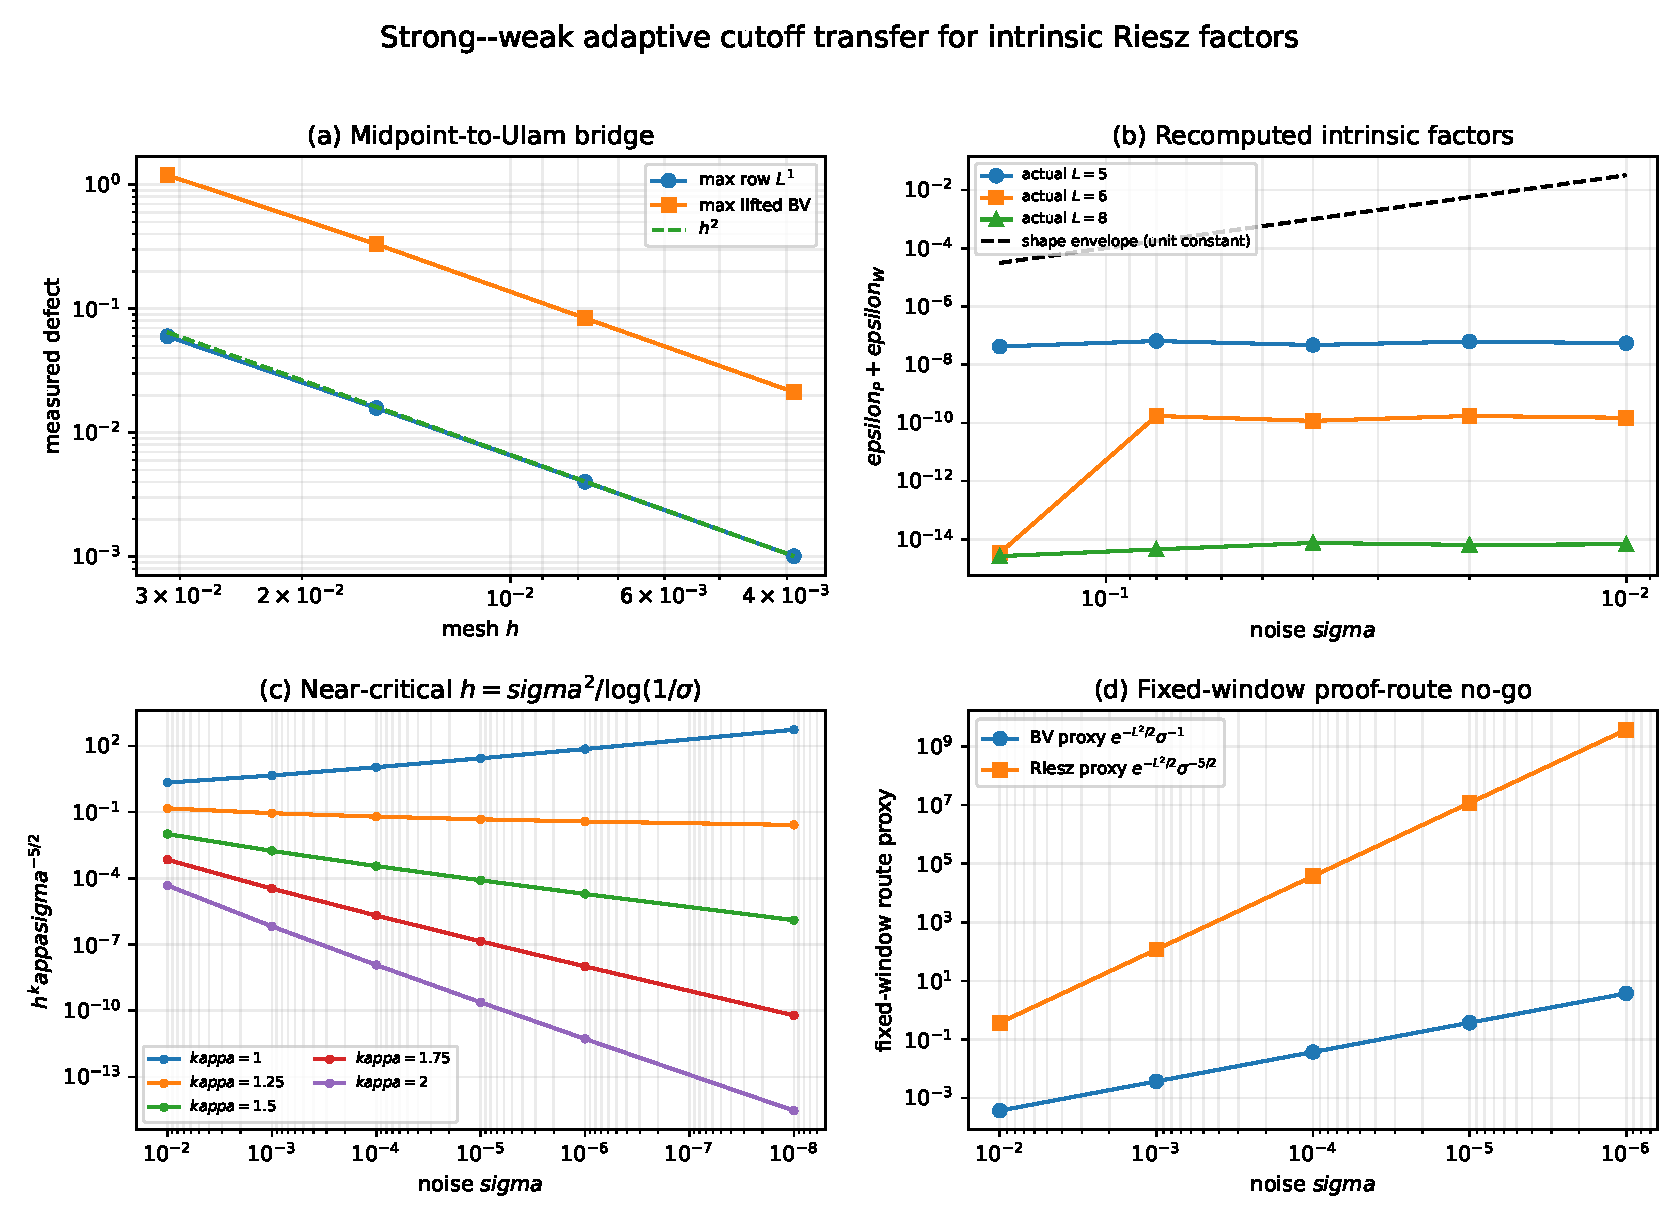
\includegraphics[width=\textwidth]{figures/strong_weak_riesz_cutoff_transfer.pdf}
\caption{Strong--weak cutoff audit.  (a) Midpoint--Ulam defects.  (b)
Recomputed intrinsic factors inherited from RH-54.  (c) Shape-aware
adaptive power envelopes on a near-critical mesh schedule.  (d) Growth of
the fixed-window strong--BV proof proxies.}
\label{fig:audit}
\end{figure}

\subsection{Outward-rounded scalar ledger}

A separate 256-bit Arb run evaluates the RH-39 omitted-mass formula at
$(n,\sigma,L)=(512,0.01,5)$ and obtains
\[
 Q_h\le4.965522022961893\times10^{-7}.
\]
It then composes interval inputs through all three terms of
\eqref{eq:D} and both contour weights.  Finally, at the illustrative
adaptive point $h=10^{-12}$, $\sigma=10^{-5}$, $\kappa=2$, it certifies
the unit-constant shape envelope divided by $\sqrt\sigma$ to be
$10^{-9}$.  Arb guarantees outward arithmetic for these scalar formulas
\citep{Johansson2017,Rump2010}.  The strong resolvent constants in that
small audit are illustrative inputs; no production folded-Gaussian interval
eigensolver is claimed.

\section{Consequence for the program}

RH-54's factor-aware theorem consumes separate Markov, unweighted-projector,
weighted-Riesz, and normalized-coupling defects.  The Markov and coupling
parts were already controlled by RH-39, RH-53, and RH-54.  The present
theorem supplies the two missing intrinsic-factor defects on exactly the
same adaptive family.

\begin{corollary}[Adaptive factor-aware cutoff closure]
\label{cor:rh54-closure}
On every $h=o(\sigma^2)$ schedule, RH-39's adaptive choice
$L(h)=\max\{5,2\sqrt{\log(1/h)}\}$ gives vanishing full-versus-sparse
unweighted and weighted peripheral Riesz defects.  In fact their sum is
$o(\sigma^{3/2})$.  Therefore the analytic Riesz/cutoff premise in the
RH-54 factor-aware intrinsic Hardy-triple transfer is satisfied.
\end{corollary}

The resulting status is:
\begin{description}[leftmargin=4.8cm,style=nextline]
 \item[Midpoint--Ulam interface]
 Closed analytically on the adopted $h=o(\sigma^2)$ schedule.

 \item[Adaptive intrinsic Riesz modulus]
 Closed analytically for both projector and weighted term.  No global
 uniform $L^2$ contour is used.

 \item[Stage A3 analytic factor transfer]
 Closed: the canonical full Gaussian family transfers to the adaptive
 sparse family through recomputed intrinsic factors.

 \item[Stage A3 production interval program]
 Not closed: the largest all-column traces and intrinsic factors have not
 been executed together in interval arithmetic.

 \item[Stage A1 Hardy--Stein budget]
 Open: no theorem yet gives a dyadically uniform/polylogarithmic trace
 budget for both directional Hardy energies.

 \item[Stage A4 intrinsic identification]
 Still conditional on Stage A1.  This paper removes the Riesz/cutoff wall,
 not the Hardy wall.
\end{description}

The next focused question is therefore the uniform growing-horizon
Hardy--Stein trace budget, without revisiting global $L^2$ conditioning.

\subsection{No arithmetic or Hilbert--P\'olya conclusion}

Nothing here supplies an arithmetic trace formula, a von Mangoldt or
prime-power identity, a zeta-zero spectral identity, a self-adjoint
Hilbert--P\'olya operator, or a $T\log T$ counting law.  No
Riemann-hypothesis conclusion is drawn.  The independent TPC twin-prime
branch is not an assumption in this argument.

\section{Reproducibility and exact boundary}

The archive contains the theorem algebra in \path{src/riesz_cutoff}, the
midpoint--Ulam and inherited-factor pilot, the Arb scalar audit, machine-
readable certificate, figure, tests, dependency hashes, and manuscript.
Principal commands are:
\begin{verbatim}
PYTHONDONTWRITEBYTECODE=1 /root/math/.venv/bin/pytest -q -p no:cacheprovider
PYTHONDONTWRITEBYTECODE=1 /root/math/.venv/bin/python \
  experiments/run_riesz_cutoff_pilot.py
PYTHONDONTWRITEBYTECODE=1 /root/math/.venv/bin/python \
  experiments/run_arb_riesz_ledger.py
PYTHONDONTWRITEBYTECODE=1 /root/math/.venv/bin/python \
  experiments/build_riesz_cutoff_certificate.py
MPLBACKEND=Agg PYTHONDONTWRITEBYTECODE=1 /root/math/.venv/bin/python \
  experiments/make_figures.py
latexmk -pdf -interaction=nonstopmode -halt-on-error main.tex
\end{verbatim}

The sandwiched functional calculus, midpoint--Ulam scales, contour
inheritance, adaptive exponent theorems, and fixed-window route no-go are
analytic.  The midpoint quadrature, eigensolver defects, and fitted visual
slopes are binary64 diagnostics.  The Arb execution validates only the
reported scalar arithmetic.  These distinctions are part of the theorem
statement, not implementation caveats.

\bibliographystyle{plainnat}
\bibliography{references}
\end{document}
